\documentclass{beamer}
% =============================================================================
% ENCODING
% =============================================================================
\usepackage[utf8]{inputenc}  % UTF-8 encoding support

% =============================================================================
% GRAPHICS
% =============================================================================
\usepackage{graphicx}  % For \includegraphics (401 uses across lectures)

% =============================================================================
% MATH PACKAGES
% =============================================================================
\usepackage{amsmath}    % For align, multline, equation environments (heavily used)
\usepackage{amsfonts}   % For \mathbb (e.g., \bbR, \bbE)
\usepackage{amssymb}    % For additional math symbols

% =============================================================================
% TABLES
% =============================================================================
\usepackage{booktabs}   % For \toprule, \midrule, \bottomrule (used in lecture13, lecture14)

% =============================================================================
% LISTS
% =============================================================================
\usepackage{enumerate}  % Enhanced enumerate environment (76 uses across lectures)

% =============================================================================
% TIKZ (DIAGRAMS)
% =============================================================================
\usepackage{tikz}       % For taxonomy diagram and footnotes positioning

% =============================================================================
% UTILITY PACKAGES
% =============================================================================
\usepackage{multido}    % For \multido command used in \eqpause
\usepackage{etoolbox}   % For \AtEndEnvironment, \ifbool, \newbool (used in preamble and taxonomy)
\usepackage{xspace}     % For smart spacing after custom commands (\ODESolve, \SDESolve)

% =============================================================================
% BEAMER THEME SETTINGS
% =============================================================================
\usetheme{default}
\usecolortheme{default}

\setbeamerfont{title}{size=\Huge}
\setbeamertemplate{footline}[frame number]{}
\setbeamertemplate{section in toc}[sections numbered]

\makeatletter
\newcommand\HUGE{\@setfontsize\Huge{35}{40}}
\makeatother    

\setbeamerfont{title}{size=\HUGE}
\beamertemplatenavigationsymbolsempty

% =============================================================================
% TIKZ LIBRARIES
% =============================================================================
% Used for taxonomy diagram: arrows, positioning, shapes
\usetikzlibrary{arrows.meta,calc,shapes,positioning,shadows,trees}

% =============================================================================
% CUSTOM FOOTNOTE COMMANDS
% =============================================================================
% \myfootnote{text} - creates a footnote at the bottom of the slide
\newcommand\myfootnote[1]{%
  \vspace{-0.5cm}%
  \tikz[remember picture,overlay]
  \draw (current page.south west) +(1in + \oddsidemargin,0.5em)
  node[anchor=south west,inner sep=0pt]{\parbox{\textwidth}{%
      \rlap{\rule{10em}{0.4pt}}\raggedright\scriptsize \textit{#1}}};}

% \myfootnotewithlink{url}{text} - creates a clickable footnote (623 uses across lectures)
\newcommand\myfootnotewithlink[2]{%
  \vspace{-0.5cm}%
  \tikz[remember picture,overlay]
  \draw (current page.south west) +(1in + \oddsidemargin,0.5em)
  node[anchor=south west,inner sep=0pt]{\parbox{\textwidth}{%
      \rlap{\rule{10em}{0.4pt}}\raggedright\scriptsize\href{#1}{\textit{#2}}}};}

% =============================================================================
% SECTION/SUBSECTION OUTLINE AUTOMATION
% =============================================================================
% Automatically show outline at the beginning of each section
\AtBeginSection[]
      {
      	\begin{frame}{Outline}
      		\tableofcontents[currentsection]
      	\end{frame}
      }
      \AtBeginSubsection[]{
      	\begin{frame}{Outline}
      		\tableofcontents[currentsection,currentsubsection]
      	\end{frame}
}

% =============================================================================
% CUSTOM SLIDE ANIMATION COMMANDS
% =============================================================================
% These commands enable step-by-step reveal of equations and content
% Used heavily across all lectures (1130+ uses of \nextonslide and \eqpause)

\newcounter{noscounter}   % Counter for \nextonslide (resets on each new slide)
\newcounter{pcounter}     % Counter for pause commands (resets after \eqpause)
\newcounter{diffcounter}  % Counts pauses after equations

% \nextonslide{content} - reveals content on the next overlay
\newcommand{\nextonslide}[1]{%
  \stepcounter{noscounter}%
  \stepcounter{pcounter}%
  \stepcounter{diffcounter}%
  \onslide<\value{noscounter}->{#1}%
}

% \resetonslide - resets all animation counters (called at each frame)
\newcommand{\resetonslide}{%
    \setcounter{noscounter}{1}%
    \setcounter{pcounter}{1}%
    \setcounter{diffcounter}{0}%
}

% \eqpause - pause after equation that syncs with \nextonslide
\newcommand{\eqpause}{%
  \multido{\i=1+1}{\value{pcounter}}{\pause}%
  \stepcounter{noscounter}%
  \setcounter{pcounter}{1}%
}

% \eqpausediff - helper command, runs automatically after math environments
\newcommand{\eqpausediff}{%
  \multido{\i=1+1}{\value{diffcounter}}{\pause}%
  \addtocounter{pcounter}{-\value{diffcounter}}%
  \setcounter{diffcounter}{0}%
}

% Apply \eqpausediff after math environments
\newcommand\AtEndBoth[2]{%
  \AtEndEnvironment{#1}{#2}%
  \AtEndEnvironment{#1*}{#2}%
}

\AtEndBoth{align}{\eqpausediff}
\AtEndBoth{equation}{\eqpausediff}
\AtEndBoth{multline}{\eqpausediff}

% Reset counters at the beginning of each frame
\addtobeamertemplate{frametitle}{\resetonslide}{}

% =============================================================================
% INCLUDE OTHER CONFIGURATION FILES
% =============================================================================
% ==============================================================================
% Custom LaTeX Commands for Deep Generative Models Course
% ==============================================================================

% ==============================================================================
% BOLD LETTERS (mathbf / boldsymbol)
% ==============================================================================

% ------------------------------------------------------------------------------
% Latin Bold Lowercase
% Usage: \bx for x in bold, commonly used for vectors
% ------------------------------------------------------------------------------
\newcommand{\ba}{\mathbf{a}}
\newcommand{\bc}{\mathbf{c}}
\newcommand{\be}{\mathbf{e}}
\newcommand{\bff}{\mathbf{f}}  % Note: \bf is reserved for bold font switching
\newcommand{\bg}{\mathbf{g}}
\newcommand{\bh}{\mathbf{h}}
\newcommand{\bp}{\mathbf{p}}
\newcommand{\bq}{\mathbf{q}}
\newcommand{\bs}{\mathbf{s}}
\newcommand{\bt}{\mathbf{t}}
\newcommand{\bu}{\mathbf{u}}
\newcommand{\bv}{\mathbf{v}}
\newcommand{\bw}{\mathbf{w}}
\newcommand{\bx}{\mathbf{x}}
\newcommand{\by}{\mathbf{y}}
\newcommand{\bz}{\mathbf{z}}
\newcommand{\bzero}{\boldsymbol{0}}  % Zero vector
\newcommand{\bone}{\mathbf{1}}       % Ones vector

% ------------------------------------------------------------------------------
% Latin Bold Uppercase
% Usage: \bX for X in bold, commonly used for matrices or random vectors
% ------------------------------------------------------------------------------
\newcommand{\bA}{\mathbf{A}}
\newcommand{\bG}{\mathbf{G}}
\newcommand{\bI}{\mathbf{I}}
\newcommand{\bJ}{\mathbf{J}}
\newcommand{\bL}{\mathbf{L}}
\newcommand{\bM}{\mathbf{M}}
\newcommand{\bP}{\mathbf{P}}
\newcommand{\bQ}{\mathbf{Q}}
\newcommand{\bR}{\mathbf{R}}
\newcommand{\bT}{\mathbf{T}}
\newcommand{\bU}{\mathbf{U}}
\newcommand{\bV}{\mathbf{V}}
\newcommand{\bW}{\mathbf{W}}
\newcommand{\bX}{\mathbf{X}}
\newcommand{\bZ}{\mathbf{Z}}

% ------------------------------------------------------------------------------
% Greek Bold Lowercase
% Usage: \btheta for θ in bold, commonly used for parameter vectors
% ------------------------------------------------------------------------------
\newcommand{\bepsilon}{\boldsymbol{\epsilon}}
\newcommand{\blambda}{\boldsymbol{\lambda}}
\newcommand{\bmu}{\boldsymbol{\mu}}
\newcommand{\bphi}{\boldsymbol{\phi}}
\newcommand{\bpi}{\boldsymbol{\pi}}
\newcommand{\bpsi}{\boldsymbol{\psi}}
\newcommand{\bsigma}{\boldsymbol{\sigma}}
\newcommand{\btheta}{\boldsymbol{\theta}}

% ------------------------------------------------------------------------------
% Greek Bold Uppercase
% Usage: \bSigma for Σ in bold, commonly used for covariance matrices
% ------------------------------------------------------------------------------
\newcommand{\bPhi}{\boldsymbol{\Phi}}
\newcommand{\bSigma}{\boldsymbol{\Sigma}}
\newcommand{\bTheta}{\boldsymbol{\Theta}}

% ==============================================================================
% CALLIGRAPHIC LETTERS (mathcal)
% Usage: \cX for calligraphic X, commonly used for sets and spaces
% ==============================================================================
\newcommand{\cF}{\mathcal{F}}
\newcommand{\cI}{\mathcal{I}}
\newcommand{\cL}{\mathcal{L}}
\newcommand{\cM}{\mathcal{M}}
\newcommand{\cN}{\mathcal{N}}
\newcommand{\cO}{\mathcal{O}}
\newcommand{\cP}{\mathcal{P}}
\newcommand{\cS}{\mathcal{S}}
\newcommand{\cT}{\mathcal{T}}
\newcommand{\cW}{\mathcal{W}}
\newcommand{\cX}{\mathcal{X}}
\newcommand{\cZ}{\mathcal{Z}}

% ==============================================================================
% BLACKBOARD BOLD LETTERS (mathbb)
% Usage: \bbR for ℝ, commonly used for number sets and expectations
% ==============================================================================
\newcommand{\bbE}{\mathbb{E}}  % Expectation
\newcommand{\bbI}{\mathbb{I}}  % Indicator function
\newcommand{\bbP}{\mathbb{P}}  % Probability measure
\newcommand{\bbR}{\mathbb{R}}  % Real numbers

% ==============================================================================
% MATH OPERATORS
% ==============================================================================

% ------------------------------------------------------------------------------
% Optimization Operators
% Usage: \argmin_{x} f(x) for proper spacing and limits placement
% ------------------------------------------------------------------------------
\DeclareMathOperator*{\argmin}{arg\,min}
\DeclareMathOperator*{\argmax}{arg\,max}

% ------------------------------------------------------------------------------
% Statistical Operators
% Usage: \cov(X, Y) for covariance
% ------------------------------------------------------------------------------
\DeclareMathOperator{\cov}{cov}

% ------------------------------------------------------------------------------
% Linear Algebra Operators
% Usage: \tr(\bA) for trace of matrix A
% ------------------------------------------------------------------------------
\DeclareMathOperator{\tr}{tr}

% ------------------------------------------------------------------------------
% Other Mathematical Operators
% ------------------------------------------------------------------------------
\DeclareMathOperator{\diver}{div}      % Divergence (vector calculus)
\newcommand{\sg}{\mathrm{sg}}          % Stop-gradient operator
\DeclareMathOperator{\softmax}{softmax}
\DeclareMathOperator{\supp}{supp}      % Support of a distribution

% ==============================================================================
% PROBABILITY DISTRIBUTIONS
% Usage: X \sim \cN(0, 1), Y \sim \Bern(p)
% ==============================================================================
\DeclareMathOperator{\Bern}{Bern}      % Bernoulli distribution
\DeclareMathOperator{\Cat}{Cat}        % Categorical distribution
\DeclareMathOperator{\Gumbel}{Gumbel}  % Gumbel distribution
\DeclareMathOperator{\Uniform}{Uniform}

% ==============================================================================
% METRICS AND DIVERGENCES
% Usage: \KL(p \| q), \JSD(p, q)
% ==============================================================================
\newcommand{\Ent}{\mathrm{H}}          % Entropy
\newcommand{\FID}{\mathrm{FID}}        % Fréchet Inception Distance
\newcommand{\JSD}{D_\mathrm{JS}}        % Jensen-Shannon Divergence
\newcommand{\KL}{D_\mathrm{KL}}        % Kullback-Leibler Divergence
\DeclareMathOperator{\MMD}{MMD}        % Maximum Mean Discrepancy
\DeclareMathOperator{\SNR}{SNR}        % Signal-to-Noise Ratio

% ==============================================================================
% NEURAL NETWORK NOTATION
% ==============================================================================

% ------------------------------------------------------------------------------
% Network Architectures (upright font for abbreviations)
% Usage: f_{\btheta} = \NN_{\btheta}(\bx)
% ------------------------------------------------------------------------------
\newcommand{\MLP}{\mathrm{MLP}}        % Multi-Layer Perceptron
\newcommand{\NN}{\mathrm{NN}}          % Neural Network
\newcommand{\RNN}{\mathrm{RNN}}        % Recurrent Neural Network

% ------------------------------------------------------------------------------
% Numerical Solvers (monospace font)
% Usage: \bx_T = \ODESolve(v, \bx_0, T)
% ------------------------------------------------------------------------------
\newcommand{\ODESolve}{\texttt{ODESolve}\xspace}
\newcommand{\SDESolve}{\texttt{SDESolve}\xspace}

% ==============================================================================
% COMMON SHORTCUTS
% Usage: Frequently used subscripted or parameterized expressions
% ==============================================================================
\newcommand{\pd}{p_{\text{data}}}              % Data distribution
\newcommand{\pt}{p_{\boldsymbol{\theta}}}      % Parameterized distribution
\newcommand{\qagg}{q_{\text{agg}}}             % Aggregated posterior
\newcommand{\lambdamax}{\lambda_{\text{max}}}  % Maximum eigenvalue
  % Math shorthand commands (\bx, \bbE, \KL, etc.)
\input{../utils/title}        % Title page template
% For each possible node, we create a boolean
\newbool{hl@root}
\newbool{hl@explicit}
\newbool{hl@implicit}
\newbool{hl@exact}
\newbool{hl@approx}
\newbool{hl@gan}
\newbool{hl@ar}
\newbool{hl@nf}
\newbool{hl@vae}
\newbool{hl@score}
\newbool{hl@cont}
\newbool{hl@ddpm}
\newbool{hl@sm}
\newbool{hl@ode}
\newbool{hl@sde}
\newbool{hl@fm}

% Command to reset all bools
\newcommand{\resetAllHighlights}{%
    \boolfalse{hl@root}%
    \boolfalse{hl@explicit}%
    \boolfalse{hl@implicit}%
    \boolfalse{hl@exact}%
    \boolfalse{hl@approx}%
    \boolfalse{hl@gan}%
    \boolfalse{hl@ar}%
    \boolfalse{hl@nf}%
    \boolfalse{hl@vae}%
    \boolfalse{hl@score}%
    \boolfalse{hl@cont}%
    \boolfalse{hl@ddpm}%
    \boolfalse{hl@sm}%
    \boolfalse{hl@ode}%
    \boolfalse{hl@sde}%
    \boolfalse{hl@fm}%
}

% Command to set a single highlight
\newcommand{\setHighlight}[1]{%
    \booltrue{hl@#1}%
}

% Command to set highlights from comma-separated list
\newcommand{\setHighlights}[1]{%
    \resetAllHighlights%
    \forcsvlist{\setHighlight}{#1}%
}

% Highlighted style definition
\tikzset{
    hl/.style={line width=1.2pt, draw=black, font=\scriptsize\bfseries},
    box/.style={
        rectangle, 
        draw=gray!50, 
        rounded corners=2pt, 
        minimum width=1.9cm, 
        minimum height=0.5cm, 
        align=center, 
        font=\scriptsize, 
        line width=0.4pt
    },
    rootnode/.style={box, fill=violet!20},
    category/.style={box, fill=teal!20},
    model/.style={box, fill=yellow!30},
    arrow/.style={-Stealth, draw=gray!80, line width=0.4pt}
}

% Draw taxonomy with pre-set highlights
\newcommand{\drawTaxonomy}{%
    \begin{tikzpicture}[scale=0.9, transform shape, node distance=0.6cm and 0.3cm]
        % --- CENTRAL ROOT ---
        \ifbool{hl@root}{\node[rootnode, hl] (root) {Generative Models};}{\node[rootnode] (root) {Generative Models};}

        % --- UPPER BRANCHES ---
        \ifbool{hl@explicit}{\node[category, hl, above left=0.6cm and 0.5cm of root] (explicit) {Explicit density};}{\node[category, above left=0.6cm and 0.5cm of root] (explicit) {Explicit density};}
        \ifbool{hl@implicit}{\node[category, hl, above right=0.6cm and 0.5cm of root] (implicit) {Implicit density};}{\node[category, above right=0.6cm and 0.5cm of root] (implicit) {Implicit density};}

        \ifbool{hl@exact}{\node[category, hl, above left=0.6cm and -0.6cm of explicit] (exact) {Exact likelihood};}{\node[category, above left=0.6cm and -0.6cm of explicit] (exact) {Exact likelihood};}
        \ifbool{hl@approx}{\node[category, hl, above right=0.6cm and -0.6cm of explicit] (approx) {Approximate likelihood};}{\node[category, above right=0.6cm and -0.6cm of explicit] (approx) {Approximate likelihood};}

        \ifbool{hl@gan}{\node[model, hl, above=0.6cm of implicit] (gans) {GANs};}{\node[model, above=0.6cm of implicit] (gans) {GANs};}

        \ifbool{hl@ar}{\node[model, hl, above left=0.6cm and -0.9cm of exact] (ar) {Autoregressive \\ models};}{\node[model, above left=0.6cm and -0.9cm of exact] (ar) {Autoregressive \\ models};}
        \ifbool{hl@nf}{\node[model, hl, above right=0.6cm and -0.9cm of exact] (nf) {Normalizing \\ Flows};}{\node[model, above right=0.6cm and -0.9cm of exact] (nf) {Normalizing \\ Flows};}
        \ifbool{hl@vae}{\node[model, hl, above=0.6cm of approx] (vae) {Variational \\ Autoencoders};}{\node[model, above=0.6cm of approx] (vae) {Variational \\ Autoencoders};}

        % --- LOWER BRANCHES ---
        \ifbool{hl@score}{\node[category, hl, below left=0.6cm and 0.5cm of root] (score) {Score-based};}{\node[category, below left=0.6cm and 0.5cm of root] (score) {Score-based};}
        \ifbool{hl@cont}{\node[category, hl, below right=0.6cm and 0.5cm of root] (cont) {Continuous \\ dynamics};}{\node[category, below right=0.6cm and 0.5cm of root] (cont) {Continuous \\ dynamics};}

        \ifbool{hl@sm}{\node[model, hl, below left=0.6cm and -0.8cm of score] (sm) {Score Matching};}{\node[model, below left=0.6cm and -0.8cm of score] (sm) {Score Matching};}
        \ifbool{hl@ddpm}{\node[model, hl, below right=0.6cm and -0.8cm of score] (ddpm) {Denoising Diffusion};}{\node[model, below right=0.6cm and -0.8cm of score] (ddpm) {Denoising Diffusion};}

        \ifbool{hl@ode}{\node[model, hl, below left=0.6cm and -0.8cm of cont] (ode) {Neural ODEs};}{\node[model, below left=0.6cm and -0.8cm of cont] (ode) {Neural ODEs};}
        \ifbool{hl@sde}{\node[model, hl, below right=0.6cm and -0.8cm of cont] (sde) {SDE-based \\ Diffusion};}{\node[model, below right=0.6cm and -0.8cm of cont] (sde) {SDE-based \\ Diffusion};}

        \ifbool{hl@fm}{\node[model, hl, below=0.6cm of ode] (fm) {Flow Matching};}{\node[model, below=0.6cm of ode] (fm) {Flow Matching};}

        % --- CONNECTIONS ---
        \draw[arrow] (root.north) -- ++(0,0.3) -| (explicit.south);
        \draw[arrow] (root.north) -- ++(0,0.3) -| (implicit.south);
        \draw[arrow] (root.south) -- ++(0,-0.3) -| (score.north);
        \draw[arrow] (root.south) -- ++(0,-0.3) -| (cont.north);
        \draw[arrow] (explicit.north) -- ++(0,0.3) -| (exact.south);
        \draw[arrow] (explicit.north) -- ++(0,0.3) -| (approx.south);
        \draw[arrow] (exact.north) -- ++(0,0.3) -| (ar.south);
        \draw[arrow] (exact.north) -- ++(0,0.3) -| (nf.south);
        \draw[arrow] (approx.north) -- (vae.south);
        \draw[arrow] (implicit.north) -- (gans.south);
        \draw[arrow] (score.south) -- ++(0,-0.3) -| (sm.north);
        \draw[arrow] (score.south) -- ++(0,-0.3) -| (ddpm.north);
        \draw[arrow] (cont.south) -- ++(0,-0.3) -| (ode.north);
        \draw[arrow] (cont.south) -- ++(0,-0.3) -| (sde.north);
        \draw[arrow] (ode.south) -- (fm.north);
    \end{tikzpicture}
}

% The main taxonomy rendering command
\newcommand{\renderTaxonomy}[1]{%
    \setHighlights{#1}%
    \centering
    \drawTaxonomy%
}     % Generative models taxonomy diagram

\createdgmtitle{3}

%--------------------------------------------------------------------------------
\begin{document}
%--------------------------------------------------------------------------------
\begin{frame}[noframenumbering,plain]
	\titlepage
	\resetonslide
\end{frame}
%=======
\begin{frame}{Recap of Previous Lecture}
    \begin{block}{Jacobian Matrix}
		Let $\bff: \bbR^m \rightarrow \bbR^m$ be a differentiable function.
		\[
			\bz = \bff(\bx), \quad 
			\bJ =  \frac{\partial \bz}{\partial \bx} =
			\begin{pmatrix}
				\frac{\partial z_1}{\partial x_1} & \dots & \frac{\partial z_1}{\partial x_m} \\
				\vdots & \ddots & \vdots \\ 
				\frac{\partial z_m}{\partial x_1} & \dots & \frac{\partial z_m}{\partial x_m}
			\end{pmatrix} \in \bbR^{m \times m}
		\]
		\vspace{-0.3cm}
	\end{block}
	\begin{block}{Change of Variables Theorem (CoV)}
		Let $\bx\in \bbR^m$ be a random vector with density $p(\bx)$, and let $\bff: \bbR^m \rightarrow \bbR^m$ be a $C^1$-diffeomorphism ($\bff$ and $\bff^{-1}$ are continuously differentiable mappings). 
		If $\bz = \bff(\bx)$, then
		\begin{align*}
			p(\bx) &= p(\bz) |\det(\bJ_{\bff})| = p(\bz) \left|\det \left( \frac{\partial \bz}{\partial \bx} \right) \right| 
			= p(\bff(\bx)) \left|\det \left(  \frac{\partial \bff(\bx)}{\partial \bx} \right) \right| \\
			p(\bz) &= p(\bx) |\det(\bJ_{\bff^{-1}})| = p(\bx) \left|\det \left(  \frac{\partial \bx}{\partial \bz} \right) \right| 
			= p(\bff^{-1}(\bz)) \left|\det \left(  \frac{\partial \bff^{-1}(\bz)}{\partial \bz} \right) \right|
		\end{align*}
		\vspace{-0.5cm}
	\end{block}
\end{frame}
%=======
\begin{frame}{Recap of Previous Lecture}
    \myfootnotewithlink{https://arxiv.org/abs/1605.08803}{Dinh L., Sohl-Dickstein J., Bengio S. Density Estimation Using Real NVP, 2016} 
	\begin{block}{Definition}
		A normalizing flow is a $C^1$-diffeomorphism that transforms data $\bx$ to noise $\bz$.
	\end{block}
	\vspace{-0.1cm}
	\begin{figure}
		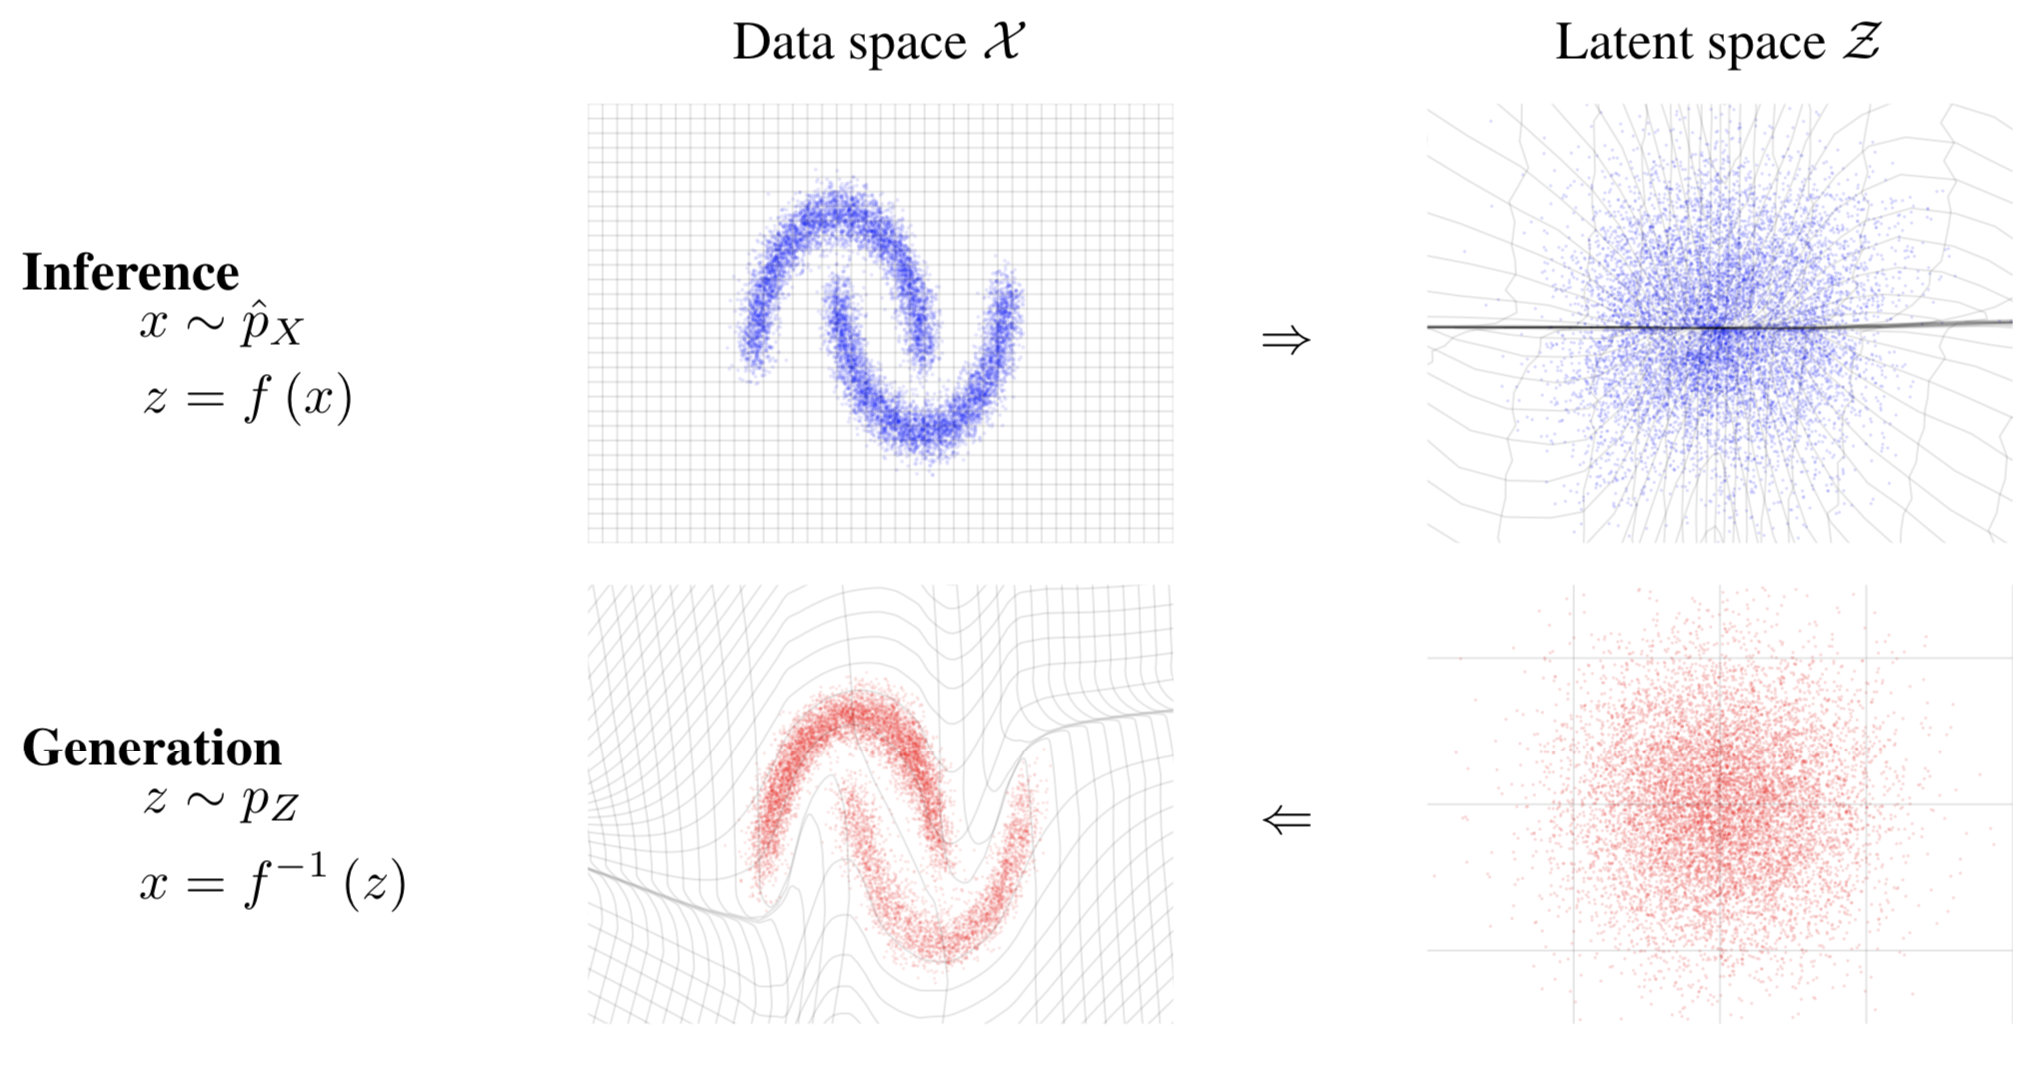
\includegraphics[width=0.85\linewidth]{figs/flows_how2}
	\end{figure}
	\vspace{-0.5cm}
	\begin{block}{Log-Likelihood}
		\vspace{-0.5cm}
		\[
			\log \pt(\bx) = \log p(\bff_K \circ \cdots \circ \bff_1(\bx)) + \sum_{k=1}^K\log |\det (\bJ_{\bff_k})|
		\]
	\end{block}
\end{frame}
%=======
\begin{frame}{Recap of Previous Lecture}
    \myfootnote{\href{https://arxiv.org/abs/1807.03039}{Kingma D. P., et al. Glow: Generative Flow With Invertible 1x1 Convolutions, 2018}  \\
	\href{https://arxiv.org/abs/1901.11137}{Hoogeboom E., et al. Emerging Convolutions for Generative Normalizing Flows, 2019}
	}
	\vspace{-0.5cm}
	\begin{block}{Flow Log-Likelihood}
		\vspace{-0.3cm}
		\[
			\log \pt(\bx) = \log p(\bff_{\btheta}(\bx)) + \log |\det (\bJ_\bff)|
		\]
		\vspace{-0.5cm}
	\end{block}
	One significant challenge is efficiently computing the Jacobian determinant.
	\begin{block}{Linear Flows}	
		\vspace{-0.2cm}
		\[
			\bz = \bff_{\btheta}(\bx) = \bW \bx, \quad \bW \in \bbR^{m \times m}, \quad \btheta = \bW, \quad \bJ_\bff = \bW^\top
		\]
	\end{block}
	\vspace{-0.3cm}
	\begin{itemize}
		\item LU Decomposition:
		\[
			\bW = \bP \bL \bU.
		\]
		\item QR Decomposition:
		\[
			\bW = \bQ \bR.
		\]
	\end{itemize}
	Decomposition is performed only once during initialization. Then the decomposed matrices ($\bP, \bL, \bU$ or $\bQ, \bR$) are optimized.
\end{frame}
%=======
\begin{frame}{Recap of Previous Lecture}
    \myfootnotewithlink{https://arxiv.org/abs/1705.07057}{Papamakarios G., Pavlakou T., Murray I. Masked Autoregressive Flow for Density Estimation, 2017} 
	Consider an autoregressive model:
	\vspace{-0.3cm}
	{\small
		\[
		\pt(\bx) = \prod_{j=1}^m \pt(x_j | \bx_{1:j - 1}), \quad
		\pt(x_j | \bx_{1:j - 1}) = \cN \left(\mu_{j, \btheta}(\bx_{1:j-1}), \sigma^2_{j, \btheta} (\bx_{1:j-1})\right).
		\]
	}
	\vspace{-0.5cm}
	\begin{block}{Gaussian Autoregressive Normalizing Flow}
		\vspace{-0.5cm}
		\begin{align*}
			\bx &= \bff^{-1}_{\btheta}(\bz) \quad \Rightarrow \quad {\color{violet} x_j} = \sigma_{j, \btheta} ({\color{violet} \bx_{1:j-1}}) \cdot {\color{teal} z_j} + \mu_{j, \btheta}({\color{violet} \bx_{1:j-1}}). \\
			\bz &= \bff_{\btheta}(\bx) \quad \Rightarrow \quad {\color{teal} z_j} = \left({\color{violet}x_j} - \mu_{j, \btheta}({\color{violet}\bx_{1:j-1}}) \right) \cdot \frac{1}{ \sigma_{j, \btheta} ({\color{violet}\bx_{1:j-1}})}.
		\end{align*}
		\vspace{-0.5cm}
	\end{block}
	\begin{itemize}
		\item This transformation is both \textbf{$C^1$-diffeomorphism}, mapping $p(\bz)$ to $\pt(\bx)$.
		\item The Jacobian matrix for this transformation is triangular.
	\end{itemize}
	The generative function $\bff^{-1}_{\btheta}(\bz)$ is \textbf{sequential}, while the inference function $\bff_{\btheta}(\bx)$ is \textbf{not sequential}.
\end{frame}
%=======
\begin{frame}{Recap of Previous Lecture}
    \myfootnotewithlink{https://arxiv.org/abs/1605.08803}{Dinh L., Sohl-Dickstein J., Bengio S. Density Estimation Using Real NVP, 2016} 

	Let us partition $\bx$ and $\bz$ into two groups: 
	\[
		\bx = [\bx_1, \bx_2] = [\bx_{1:d}, \bx_{d+1:m}]; \quad \bz = [\bz_1, \bz_2] = [\bz_{1:d}, \bz_{d+1:m}].
	\]
	\vspace{-0.7cm}
	\begin{block}{Coupling Layer}
		\vspace{-0.7cm}
		\[
			\begin{cases} {\color{violet}\bx_1} = {\color{teal}\bz_1}; \\ {\color{violet}\bx_2} = {\color{teal}\bz_2} \odot \bsigma_{\btheta}({\color{teal}\bz_1}) + \bmu_{\btheta}({\color{teal}\bz_1}).\end{cases}  
			\begin{cases} {\color{teal}\bz_1} ={\color{violet} \bx_1}; \\ {\color{teal}\bz_2} = \left({\color{violet}\bx_2} - \bmu_{\btheta}({\color{violet}\bx_1}) \right) \odot \frac{1}{\bsigma_{\btheta}({\color{violet}\bx_1})}.\end{cases}
		\]
		Both density estimation and sampling require just a single pass!
	\end{block}
	\begin{block}{Jacobian}
		\vspace{-0.3cm}
		\[
			\det \left( \frac{\partial \bz}{\partial \bx} \right) = \det 
			\begin{pmatrix}
				\bI_d & 0_{d \times (m - d)} \\
				\frac{\partial \bz_2}{\partial \bx_1} & \frac{\partial \bz_2}{\partial \bx_2}
			\end{pmatrix} = \prod_{j=1}^{m - d} \frac{1}{\sigma_{j, \btheta}(\bx_1)}.
		\]
	\end{block}
	A coupling layer is a special instance of an gaussian autoregressive normalizing flow.
\end{frame}
%=======
\section{Latent Variable Models (LVM) (continued)}
%=======
\begin{frame}{Recap of Previous Lecture}
	\begin{block}{Maximum Likelihood Estimation (MLE) Problem}
		\vspace{-0.7cm}
		\[
			\btheta^* = \argmax_{\btheta} \pt(\bX) = \argmax_{\btheta} \prod_{i=1}^n \pt(\bx_i) = \argmax_{\btheta} \sum_{i=1}^n \log \pt(\bx_i).
		\]
		\vspace{-0.5cm}
	\end{block}
	The distribution $\pt(\bx)$ should be highly complex (just like the true data distribution $\pd(\bx)$).
	\begin{block}{Latent Variable}
		Introduce a latent variable $\bz$ for each observed sample $\bx$:
		\[
			\pt(\bx, \bz) = \pt(\bx | \bz) p(\bz); \quad 
		\log \pt(\bx, \bz) = \log \pt(\bx | \bz) + \log p(\bz).
		\]
		\[
			\nextonslide{\pt(\bx) = \int \pt(\bx, \bz) d\bz = \int \pt(\bx | \bz) p(\bz) d\bz.}
		\]
	\end{block}
	\vspace{-0.3cm}
	\begin{itemize}
		\item $p(\bz)$ is prior distribution over the latent variable.
		\item $\pt(\bx | \bz)$ is \textbf{decoder} distribution.
		\item Both $\pt(\bx | \bz)$ and $p(\bz)$ are usually much simpler than $\pt(\bx)$.
	\end{itemize}
\end{frame}
%=======
\begin{frame}{Outline}
    \tableofcontents
\end{frame}
%=======
\section{Variational Evidence Lower Bound (ELBO)}
%=======
\begin{frame}{MLE for LVM}
    \myfootnotewithlink{https://jmtomczak.github.io/blog/4/4\_VAE.html}{image credit: https://jmtomczak.github.io/blog/4/4\_VAE.html}
	\[
		\sum_{i=1}^n \log \pt(\bx_i) = \sum_{i=1}^n \log \int \pt(\bx_i| \bz_i) p(\bz_i) d\bz_i \rightarrow \max_{\btheta}.
	\]
    \eqpause
	\vspace{-0.6cm}
	\begin{figure}
		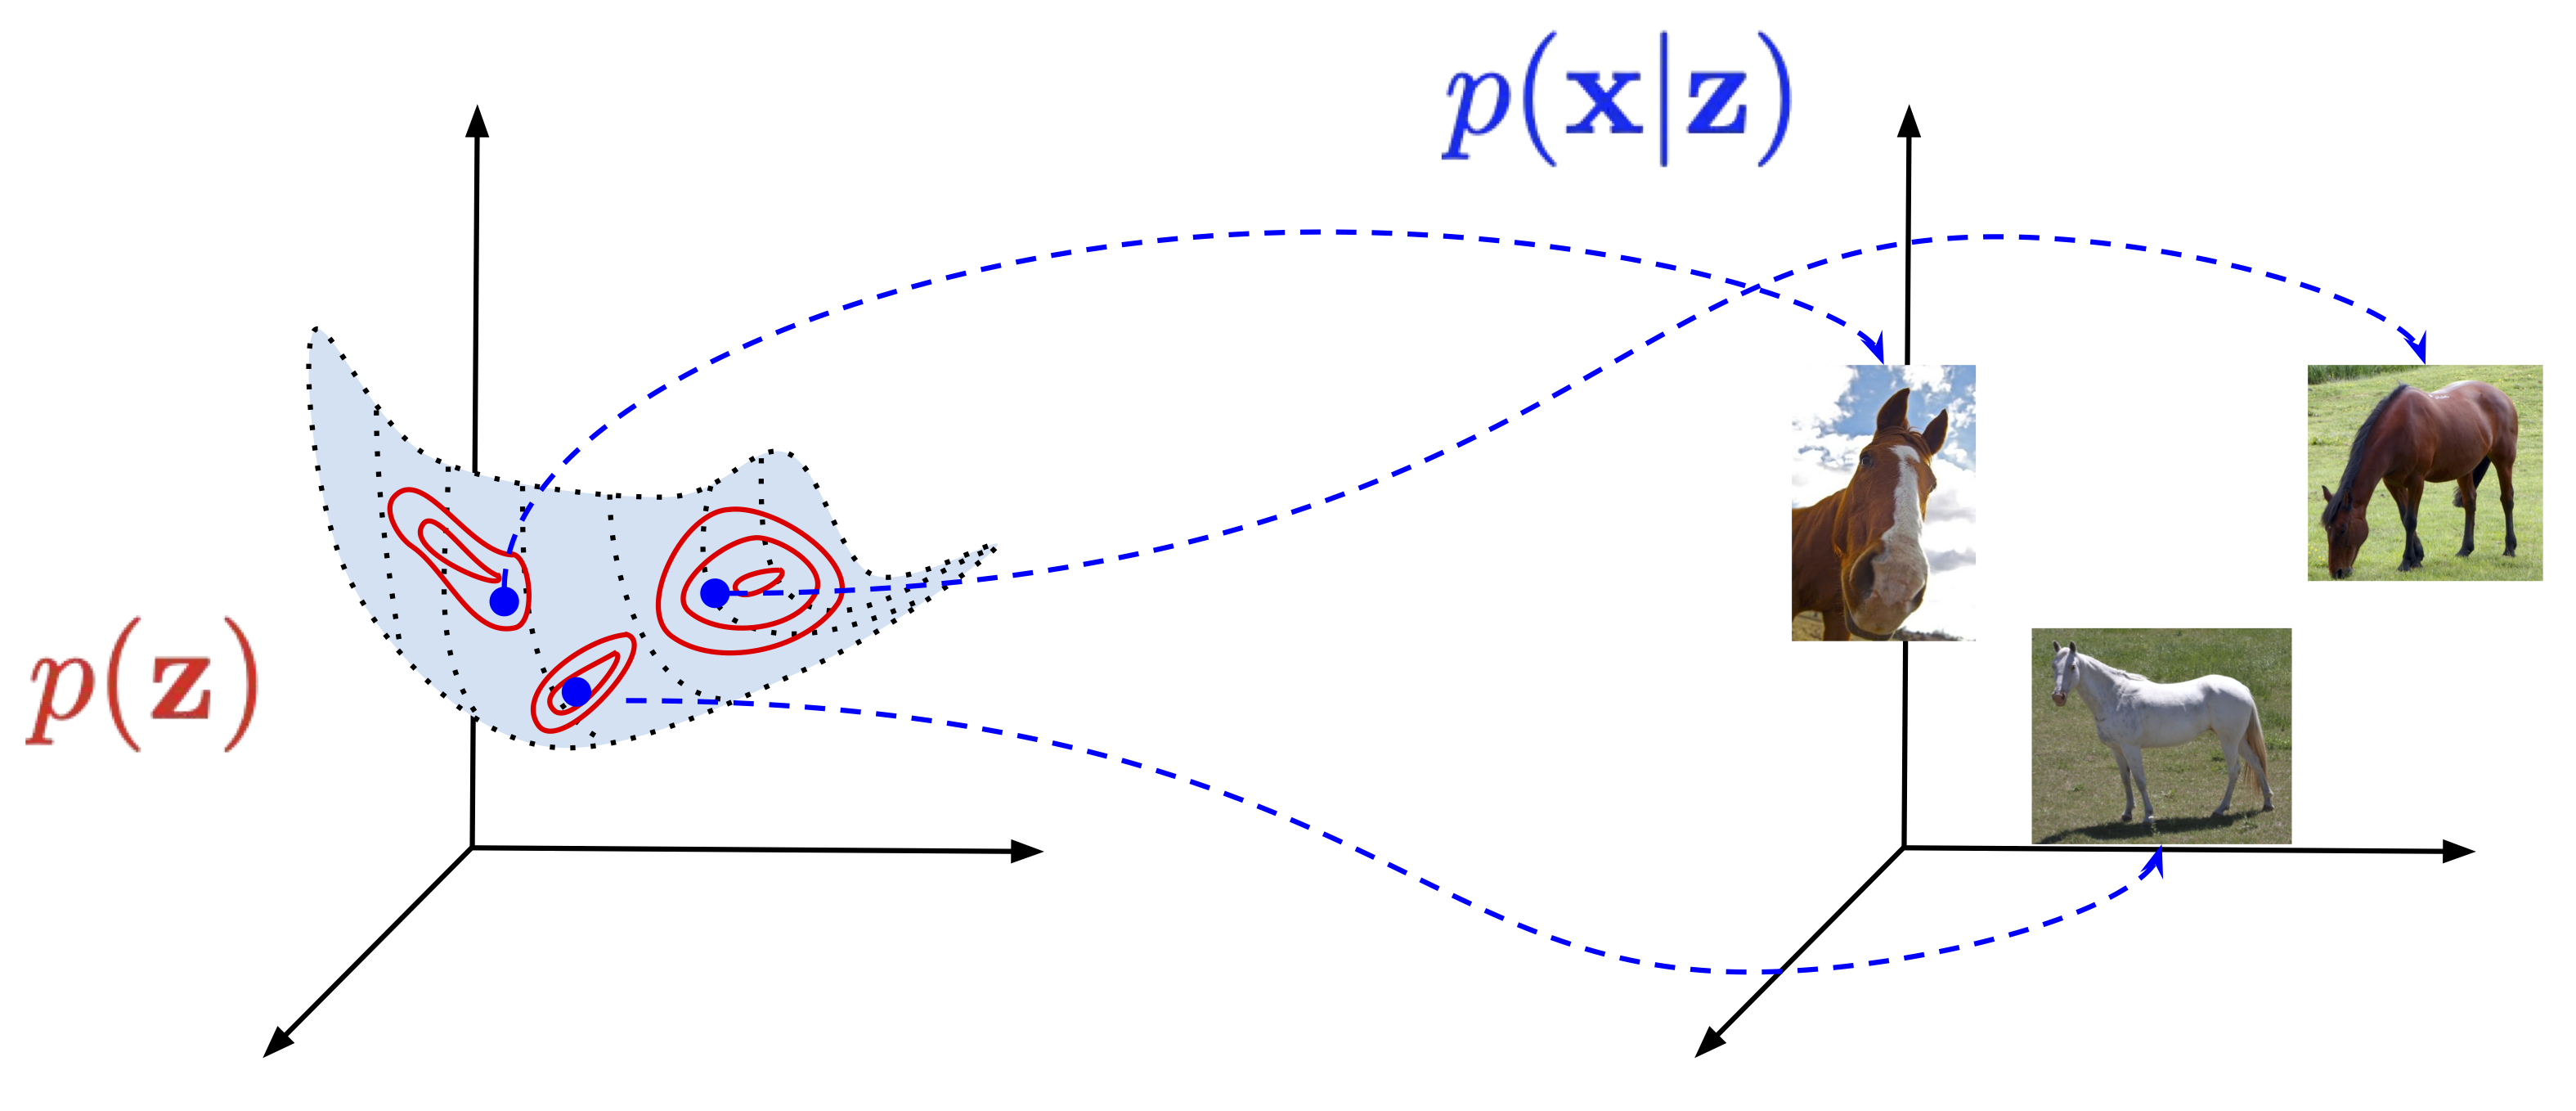
\includegraphics[width=.65\linewidth]{figs/lvm_diagram}
	\end{figure}
    \eqpause
	\vspace{-0.5cm}
	\begin{block}{Naive Monte Carlo Estimation}
		\vspace{-0.7cm}
		\[
			\log \pt(\bx) = \log \bbE_{p(\bz)} \pt(\bx | \bz) \geq \bbE_{p(\bz)} \log \pt(\bx | \bz) \approx \frac{1}{K} \sum_{k=1}^{K} \log \pt(\bx | \bz_k),
		\]
		\vspace{-0.7cm} \\
		where $\bz_k \sim p(\bz)$. \\
        \eqpause
		\textbf{Challenge:} As the dimensionality of $\bz$ increases, the number of samples needed to adequately cover the latent space grows exponentially.
	\end{block}
\end{frame}
%=======
\begin{frame}{ELBO Derivation I}
	\begin{block}{Bayes theorem}
		\vspace{-0.3cm}
		\[
			\pt(\bz | \bx) = \frac{\pt(\bx, \bz)}{\pt(\bx)} \quad \Rightarrow \quad \pt(\bx) = \frac{\pt(\bx, \bz)}{\pt(\bz | \bx)} 
		\]
		\vspace{-0.5cm}
	\end{block}
	\eqpause
	\begin{block}{Log likelihood}
		\vspace{-0.5cm}
		\begin{multline*}
			\log \pt(\bx) = \int q(\bz) \log \pt(\bx) d\bz 
			\nextonslide{= \bbE_{q} \log \left[ \frac{\pt(\bx, \bz)}{\pt(\bz | \bx)}  \right]}
			\nextonslide{= \\ = \bbE_{q} \log \left[ \frac{\pt(\bx, \bz) {\color{teal}q(\bz)}}{\pt(\bz | \bx) {\color{teal}q(\bz)}}  \right]}
			\nextonslide{= \\ = \bbE_{q}  \log \frac{\pt(\bx, \bz)}{q(\bz)} + \bbE_{q} \log \frac{q(\bz)}{\pt(\bz | \bx)}}
		\end{multline*}
		\vspace{-0.5cm}
	\end{block}
    \eqpause
	\begin{itemize}
		\item Here, $q(\bz)$ is any distribution such that $\int q(\bz) d\bz = 1$.
		\item {\color{gray} We assume that $\supp(q(\bz)) = \supp(\pt(\bz | \bx)) = \bbR^{d}$}.
	\end{itemize}
\end{frame}
%=======
\begin{frame}{ELBO Derivation II}
	\begin{block}{Variational Decomposition}
		\vspace{-0.7cm}
		\begin{multline*}
			\log \pt(\bx) = \bbE_{q}  \log \frac{\pt(\bx, \bz)}{q(\bz)} + \bbE_{q} \log \frac{q(\bz)}{\pt(\bz | \bx)}
			\nextonslide{= \\ = \cL_{q, \btheta}(\bx) + {\color{violet}\KL(q(\bz) \| \pt(\bz|\bx))}} 
			\nextonslide{\geq \cL_{q, \btheta}(\bx)}
		\end{multline*}
		\vspace{-0.5cm}
	\end{block}
	\eqpause
	\begin{block}{Variational Evidence Lower Bound (ELBO)}	
		\vspace{-0.3cm}
		\[
			\cL_{q, \btheta}(\bx) = \bbE_{q} \log \frac{\pt(\bx, \bz)}{q(\bz)}  \leq \log \pt(\bx) 
		\]
	\end{block}
	\eqpause
	\begin{itemize}
		\item This inequality holds for any choice of $q(\bz)$.
		\eqpause
		\item Instead of maximizing the likelihood, maximize the ELBO:
		\[
			\max_{\btheta} \pt(\bx) \quad \rightarrow \quad \max_{q, \btheta} \cL_{q, \btheta}(\bx)
		\]
		\eqpause
		\vspace{-0.3cm}
		\item Distribution $q(\bz)$ is treated as \textbf{variational} parameter.
	\end{itemize}
\end{frame}
%=======
\begin{frame}{Variational Evidence Lower Bound (ELBO)}
    \myfootnote{Bishop\,C. Pattern Recognition and Machine Learning, 2006}
	\[
		\log \pt(\bx) = \cL_{q, \btheta}(\bx) + \KL(q(\bz) \| \pt(\bz|\bx))
	\]
	What is the optimal distribution $q^*(\bz)$ given fixed $\btheta^*$?
    \eqpause
	\vspace{-0.3cm}
	\begin{multline*}
		q^*(\bz) = \argmax_q \cL_{q, \btheta^*}(\bx) 
		\nextonslide{= \\ = \argmin_q \KL(q(\bz) \| p_{\btheta^*}(\bz | \bx))}
		\nextonslide{= p_{\btheta^*}(\bz| \bx)}.
	\end{multline*}
	\vspace{-0.3cm} \\ 
	\eqpause
	Here we got the intuition about variational distribution $q(\bz)$ – it estimates the posterior~$p_{\btheta^*}(\bz| \bx)$.
	\vspace{-0.3cm}
    \eqpause
	\begin{minipage}[t]{0.45\columnwidth}
		\begin{figure}
			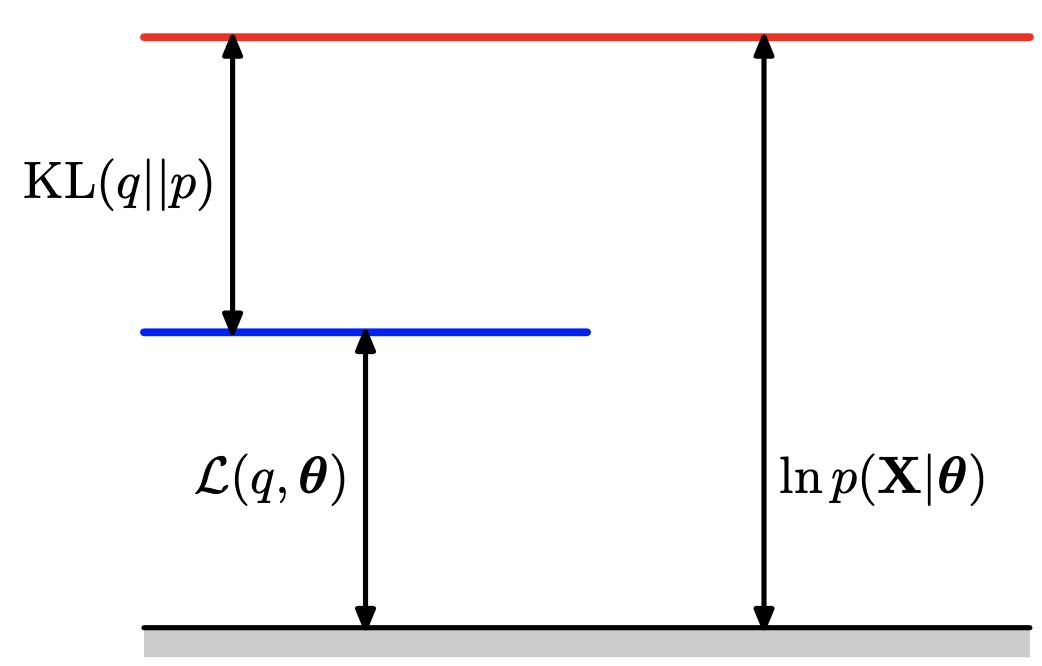
\includegraphics[width=0.9\linewidth]{figs/em_bishop1}
		\end{figure}
	\end{minipage}%
	\begin{minipage}[t]{0.55\columnwidth}
		\begin{figure}
			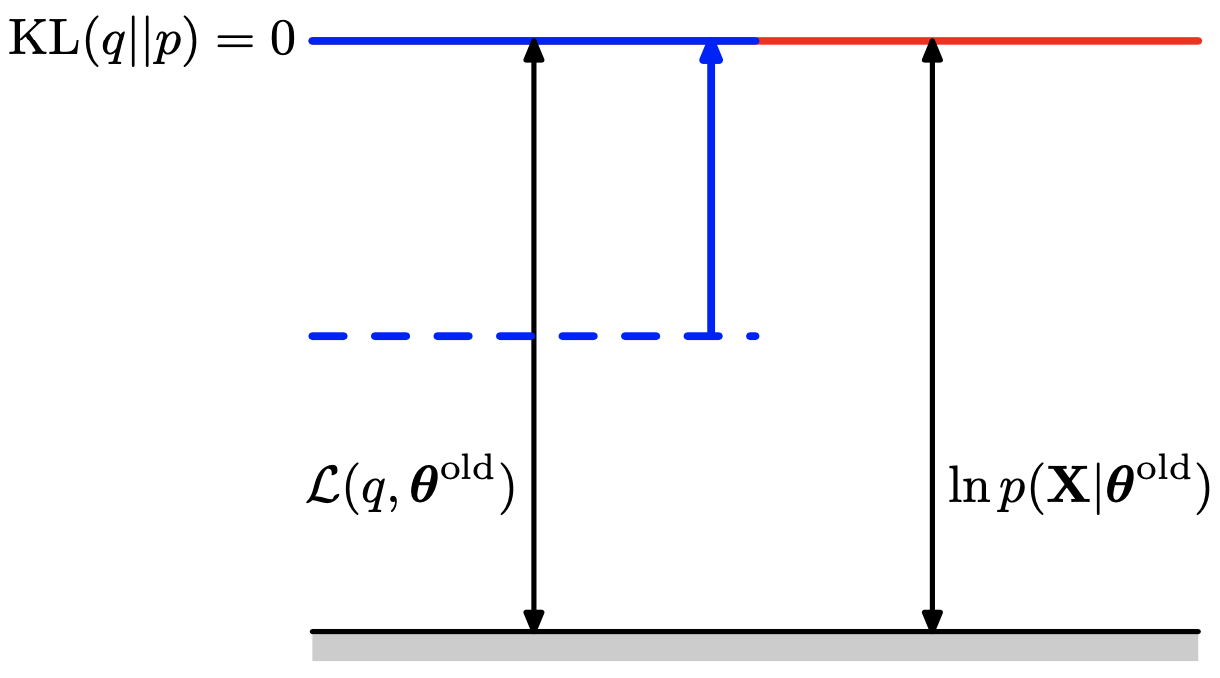
\includegraphics[width=0.85\linewidth]{figs/em_bishop2}
		\end{figure}
	\end{minipage}
\end{frame}
%=======
\begin{frame}{Variational Evidence Lower Bound (ELBO)}
	\vspace{-0.3cm}
	\begin{align*}
		\cL_{q, \btheta}(\bx) &= \int q(\bz) \log \frac{\color{violet}\pt(\bx, \bz)}{\color{teal}q(\bz)}d\bz \\ 
		\nextonslide{&= \int q(\bz) \log {\color{violet}\pt(\bx | \bz)} d\bz + \int q(\bz) \log \frac{\color{violet}p(\bz)}{\color{teal}q(\bz)}d\bz} \\ 
		\nextonslide{&= \bbE_{q} \log \pt(\bx | \bz) - \KL (q(\bz) \| p(\bz))}
	\end{align*}
    \eqpause
	\vspace{-0.5cm}
	\begin{block}{Log-Likelihood Decomposition}
		\vspace{-0.8cm}
		\begin{multline*}
			\log \pt(\bx) = {\color{olive}\cL_{q, \btheta}(\bx)} + \KL(q(\bz) \| \pt(\bz|\bx)) 
			\nextonslide{ = \\ = {\color{olive}\bbE_{q} \log \pt(\bx | \bz) - \KL (q(\bz) \| p(\bz))} + \KL(q(\bz) \| \pt(\bz|\bx)).}
		\end{multline*}
		\vspace{-0.7cm}
	\end{block}
    \eqpause
	\begin{itemize}
		\item What do we get if we drop $\KL (q(\bz) \| p(\bz))$ term from ELBO?
		\eqpause
		\item What do we have in the term $\bbE_{q} \log \pt(\bx | \bz)$ in the case of Normal distribution?
	\end{itemize}
\end{frame}
%=======
\section{Amortized Inference}
%=======
\begin{frame}{Parametric Variable Posterior}
	\begin{block}{Variational Posterior}
		\vspace{-0.3cm}
		\[
			q(\bz) = \argmax_q \cL_{q, \btheta^*}(\bx) = \argmin_q \KL(q \| p) =
		p_{\btheta^*}(\bz| \bx).
		\]
		\eqpause
		\begin{itemize}
			\item {\color{violet}$p_{\btheta^*}(\bz| \bx)$ may be \textbf{intractable}};
			\item {\color{teal}$q(\bz)$ is individual for each data point $\bx$}.
		\end{itemize}
	\end{block}
	\eqpause
	\begin{block}{Amortized Variational Inference}
		We restrict the family of possible distributions $q(\bz)$ to a parametric class $q_{\bphi}(\bz| \bx)$, {\color{teal}conditioned on data $\bx$} and {\color{violet}parameterized by $\bphi$}.
	\end{block}		
	\eqpause
	\begin{block}{Gradient Update}
		\[
			\begin{bmatrix}
				\bphi_k \\
				\btheta_k
			\end{bmatrix}
			= \left.
			\begin{bmatrix}
				\bphi_{k-1} + \eta \cdot \nabla_{\bphi} \cL_{\bphi, \btheta}(\bx) \\
				\btheta_{k-1} + \eta \cdot \nabla_{\btheta} \cL_{\bphi, \btheta}(\bx)
			\end{bmatrix}
			\right|_{(\bphi_{k-1}, \btheta_{k-1})}
		\]
	\end{block}
\end{frame}
%=======
\begin{frame}{ELBO Optimization}
	\myfootnote{Bishop C., Deep Learning: Foundations and Concepts, 2024}
	\begin{block}{Gradient Update}
		\[
			\begin{bmatrix}
				\bphi_k \\
				\btheta_k
			\end{bmatrix}
			= \left.
			\begin{bmatrix}
				\bphi_{k-1} + \eta \cdot \nabla_{\bphi} \cL_{\bphi, \btheta}(\bx) \\
				\btheta_{k-1} + \eta \cdot \nabla_{\btheta} \cL_{\bphi, \btheta}(\bx)
			\end{bmatrix}
			\right|_{(\bphi_{k-1}, \btheta_{k-1})}
		\]
	\end{block}
	\begin{figure}
		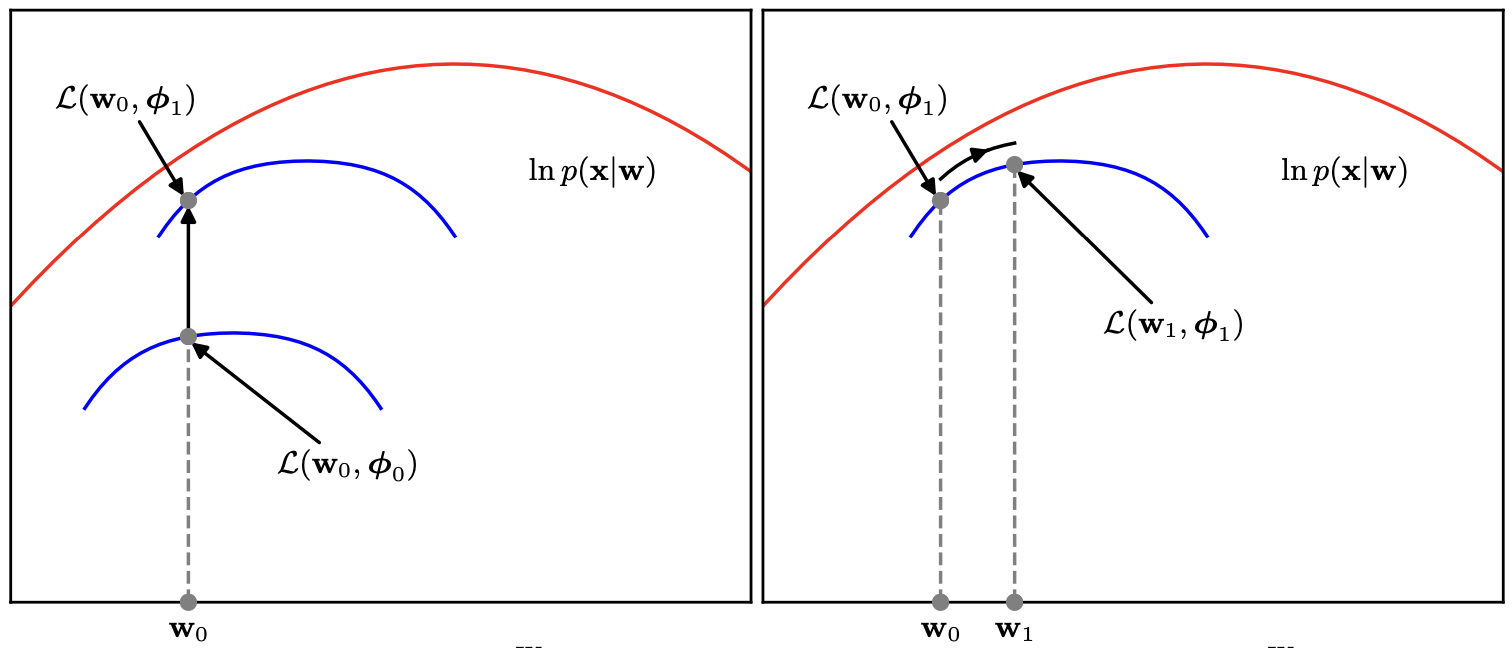
\includegraphics[width=\linewidth]{figs/em_bishop4}
	\end{figure}
		
\end{frame}
%=======
\begin{frame}{ELBO Optimization}
	\begin{block}{ELBO}
		\vspace{-0.3cm}
		\[
			\log \pt(\bx) = \cL_{\bphi, \btheta}(\bx) + \KL(q_{\bphi}(\bz| \bx) \| \pt(\bz|\bx)) \geq \cL_{\bphi, \btheta}(\bx).
		\]
		\[
		 	\cL_{\bphi, \btheta}(\bx) = \bbE_{q} \log \pt(\bx | \bz) - \KL(q_{\bphi}(\bz| \bx) \| p(\bz))
		\]
		\vspace{-0.5cm}
	\end{block}
	\eqpause
	\begin{block}{Gradient Update}
		\[
			\begin{bmatrix}
				\bphi_k \\
				\btheta_k
			\end{bmatrix}
			= \left.
			\begin{bmatrix}
				\bphi_{k-1} + \eta \cdot \nabla_{\bphi} \cL_{\bphi, \btheta}(\bx) \\
				\btheta_{k-1} + \eta \cdot \nabla_{\btheta} \cL_{\bphi, \btheta}(\bx)
			\end{bmatrix}
			\right|_{(\bphi_{k-1}, \btheta_{k-1})}
		\]
		\begin{itemize}
			\item $\bphi$ denotes the parameters of the variational posterior $q_{\bphi}(\bz| \bx)$.
			\item $\btheta$ represents the parameters of the generative model $\pt(\bx | \bz)$.
		\end{itemize}
	\end{block}
	\eqpause
	The remaining step is to obtain \textbf{unbiased} Monte Carlo estimates of the gradients: $\nabla_{\bphi} \cL_{\bphi, \btheta}(\bx)$ and $\nabla_{\btheta} \cL_{\bphi, \btheta}(\bx)$. 
\end{frame}
%=======
\section{ELBO Gradients, Reparametrization Trick}
%=======
\begin{frame}{ELBO Gradients: $\nabla_{\btheta} \cL_{\bphi, \btheta}(\bx)$}
	\myfootnotewithlink{https://jmtomczak.github.io/blog/4/4\_VAE.html}{image credit: https://jmtomczak.github.io/blog/4/4\_VAE.html}
	\vspace{-0.3cm}
	\[
	 	\cL_{\bphi, \btheta}(\bx) = \bbE_{q} \log \pt(\bx | \bz) - \KL (q_{\bphi}(\bz| \bx) \| p(\bz))
	\]
	\vspace{-0.5cm}
	\eqpause
	\begin{block}{Gradient $\nabla_{\btheta} \cL_{\bphi, \btheta}(\bx)$}
		\vspace{-0.7cm}
		\begin{align*}
			\nabla_{\btheta} \cL_{\bphi, \btheta}(\bx)
			&= {\color{olive}\nabla_{\btheta}} \int q_{\bphi}(\bz| \bx) \log \pt(\bx| \bz) d \bz 
			\nextonslide{\\ &= \int q_{\bphi}(\bz| \bx) {\color{olive}\nabla_{\btheta}} \log \pt(\bx| \bz) d \bz}
			\nextonslide{\\ &\approx \nabla_{\btheta}\log \pt(\bx|\bz^*), \quad \bz^* \sim q_{\bphi}(\bz| \bx).}
		\end{align*}
		\vspace{-0.9cm}
	\end{block}
	\eqpause
	\begin{block}{Naive Monte Carlo Estimation}
		\vspace{-0.7cm}
		\[
			\log \pt(\bx) \geq \int \log \pt(\bx | \bz) p(\bz) d\bz \approx \frac{1}{K} \sum_{k=1}^{K} \log \pt(\bx | \bz_k), \quad \bz_k \sim p(\bz).
		\]
		\vspace{-0.5cm} 
	\end{block}
	\eqpause
	The variational posterior $q_{\bphi}(\bz| \bx)$ typically concentrates more probability mass in a much smaller region than the prior $p(\bz)$. 
\end{frame}
%=======
\begin{frame}{ELBO Gradients: $\nabla_{\bphi} \cL_{\bphi, \btheta}(\bx)$}
	\begin{block}{Gradient $\nabla_{\bphi} \cL_{\bphi, \btheta}(\bx)$}
		Unlike the $\btheta$-gradient, the density $q_{\bphi}(\bz| \bx)$ now depends on $\bphi$, so standard Monte Carlo estimation can't be applied:
		\begin{align*}
			\nabla_{\bphi} \cL_{\bphi, \btheta}(\bx) &= {\color{olive}\nabla_{\bphi}} \int q_{\bphi}(\bz| \bx)\log \pt(\bx | \bz) d \bz - \nabla_{\bphi} \KL(q_{\bphi}(\bz| \bx) \| p(\bz)) \\
			\nextonslide{& {\color{violet}\neq} \int q_{\bphi}(\bz| \bx) {\color{olive}\nabla_{\bphi}} \log \pt(\bx | \bz) d \bz - \nabla_{\bphi} \KL(q_{\bphi}(\bz| \bx) \| p(\bz))}
		\end{align*}
	\end{block}
	\eqpause
	\vspace{-0.5cm}
	\begin{block}{Reparametrization Trick (LOTUS Trick)} 
		Assume $\bz \sim q_{\bphi}(\bz| \bx)$ is generated by a random variable $\bepsilon \sim p(\bepsilon)$ via a deterministic mapping $\bz = \bg_{\bphi}(\bx, \bepsilon)$. Then,
		\[
			\bbE_{\bz \sim q_{\bphi}(\bz| \bx)} \bff(\bz) = \bbE_{\bepsilon \sim p(\bepsilon)} \bff(\bg_{\bphi}(\bx, \bepsilon))
		\]
		\eqpause
		\textbf{Note:} The LHS expectation is with respect to the parametric distribution $q_{\bphi}(\bz| \bx)$, while the RHS is for the non-parametric $p(\bepsilon)$.
	\end{block}
\end{frame}
%=======
\begin{frame}{ELBO Gradients: $\nabla_{\bphi} \cL_{\bphi, \btheta}(\bx)$}
	\begin{block}{Reparametrization Trick (LOTUS Trick)} 
		\vspace{-0.7cm}
		\begin{multline*}
			\nabla_{\bphi}\int q_{\bphi}(\bz| \bx) \bff(\bz) d\bz = {\color{olive}\nabla_{\bphi}} \int p(\bepsilon)  \bff(\bg_{\bphi}(\bx, \bepsilon)) d\bepsilon 
			\nextonslide{= \\ = \int p(\bepsilon) {\color{olive}\nabla_{\bphi}} \bff(\bg_{\bphi}(\bx, \bepsilon)) d\bepsilon \approx \nabla_{\bphi} \bff(\bg_{\bphi}(\bx, \bepsilon^*))},
		\end{multline*}
		\vspace{-0.5cm} \\
		where $\bepsilon^* \sim p(\bepsilon)$.
	\end{block}
	\eqpause
	\begin{block}{Variational Assumption} 
		\vspace{-0.3cm}
		\[
			p(\bepsilon) = \cN(0, \bI); \quad \bz = \bg_{\bphi}(\bx, \bepsilon) = \bsigma_{\bphi}(\bx) \odot \bepsilon + \bmu_{\bphi}(\bx);
		\]
		\[
			q_{\bphi}(\bz| \bx) = \cN (\bmu_{\bphi}(\bx), \bsigma^2_{\bphi}(\bx)).
		\]
		Here, $\bmu_{\bphi}(\cdot)$ and $\bsigma_{\bphi}(\cdot)$ are parameterized functions (outputs of a neural network). \\
		Thus, we can write $q_{\bphi}(\bz| \bx) = \NN_{e, \bphi}(\bx)$, the \textbf{encoder}.
	\end{block}
\end{frame}
%=======
\begin{frame}{ELBO Gradient: $\nabla_{\bphi} \cL_{\bphi, \btheta}(\bx)$}
	\vspace{-0.3cm}
	\[
		\nabla_{\bphi} \cL_{\bphi, \btheta}(\bx) = {\color{violet}\nabla_{\bphi} \int q_{\bphi}(\bz| \bx)\log \pt(\bx | \bz) d \bz} - {\color{teal}\nabla_{\bphi} \KL(q_{\bphi}(\bz| \bx) \| p(\bz))}
	\]
	\eqpause
	\vspace{-0.3cm}
	\begin{block}{Reconstruction Term}
		\vspace{-0.7cm}
		\begin{multline*}
			 {\color{violet}\nabla_{\bphi} \int q_{\bphi}(\bz| \bx)\log \pt(\bx | \bz) d \bz} = \int p(\bepsilon) \nabla_{\bphi} \log \pt(\bx | \bg_{\bphi}(\bx, \bepsilon)) d\bepsilon \approx \\
			 \approx \nabla_{\bphi} \log \pt\left(\bx | \bsigma_{\bphi}(\bx) \odot \bepsilon^* + \bmu_{\bphi}(\bx)\right), \quad \text{where } \bepsilon^* \sim \cN(0, \bI)
		\end{multline*}
		\eqpause
		\vspace{-0.5cm} \\
		The generative distribution $\pt(\bx | \bz)$ can be implemented as a neural network. \\
		We may write $\pt(\bx | \bz) = \NN_{d, \btheta}(\bz)$, called the \textbf{decoder}.
	\end{block}
	\eqpause
	\begin{block}{KL Term}
		$p(\bz)$ is the prior over latents $\bz$, typically $p(\bz) = \cN (0, \bI)$.
		\[
			{\color{teal}\nabla_{\bphi} \KL(q_{\bphi}(\bz| \bx) \| p(\bz))} = \nabla_{\bphi} \KL\left( \cN (\bmu_{\bphi}(\bx), \bsigma^2_{\bphi}(\bx)) \| \cN (0, \bI) \right)
		\]
		\eqpause
		This expression admits a closed-form analytic solution.
	\end{block}
\end{frame}
%=======
\section{Variational Autoencoder (VAE)}
%=======
\begin{frame}{Generative Models Taxonomy}
	\renderTaxonomy{vae}
\end{frame}
%=======
\begin{frame}{Variational Autoencoder (VAE)}
	\begin{block}{Training}
		\begin{enumerate}
			\item Sample $\bx \sim \pd(\bx)$ and $\bepsilon \sim p(\bepsilon)$.
			\item Reparametrize $\bz = \bg_{\bphi}(\bx, \bepsilon)$.
			\item Compute the ELBO:
			\vspace{-0.3cm}
			\[
				\cL_{\bphi, \btheta}(\bx) \approx \log \pt(\bx | \bz) - \KL(q_{\bphi}(\bz| \bx) \| p(\bz)).
			\]
			\vspace{-0.5cm}
			\item Update $\bphi$, $\btheta$ via stochastic gradient ascent.
		\end{enumerate}
	\end{block}
	\eqpause
	\begin{block}{Sampling}
		\begin{enumerate}
			\item Sample $\bz \sim p(\bz) = \cN(0, \bI)$.
			\item Generate $\bx \sim \pt(\bx | \bz)$.
		\end{enumerate}
	\end{block}
	\eqpause
	\textbf{Note:} The encoder $q_{\bphi}(\bz| \bx)$ isn't needed during generation.
\end{frame}
%=======
\begin{frame}{Variational Autoencoder}
	\myfootnote{\href{http://ijdykeman.github.io/ml/2016/12/21/cvae.html}{image credit: http://ijdykeman.github.io/ml/2016/12/21/cvae.html} \\ \href{https://arxiv.org/abs/1906.02691}{Kingma D. P., Welling M., An Introduction to Variational Autoencoders, 2019}}
	\vspace{-0.3cm}
	\[
	 	\cL_{\bphi, \btheta}(\bx) = \bbE_{q} \log \pt(\bx | \bz) - \KL (q_{\bphi}(\bz| \bx) \| p(\bz))
	\]
	\vspace{-0.7cm}
	\begin{minipage}[t]{0.6\columnwidth}
		\begin{figure}[h]
			\centering
			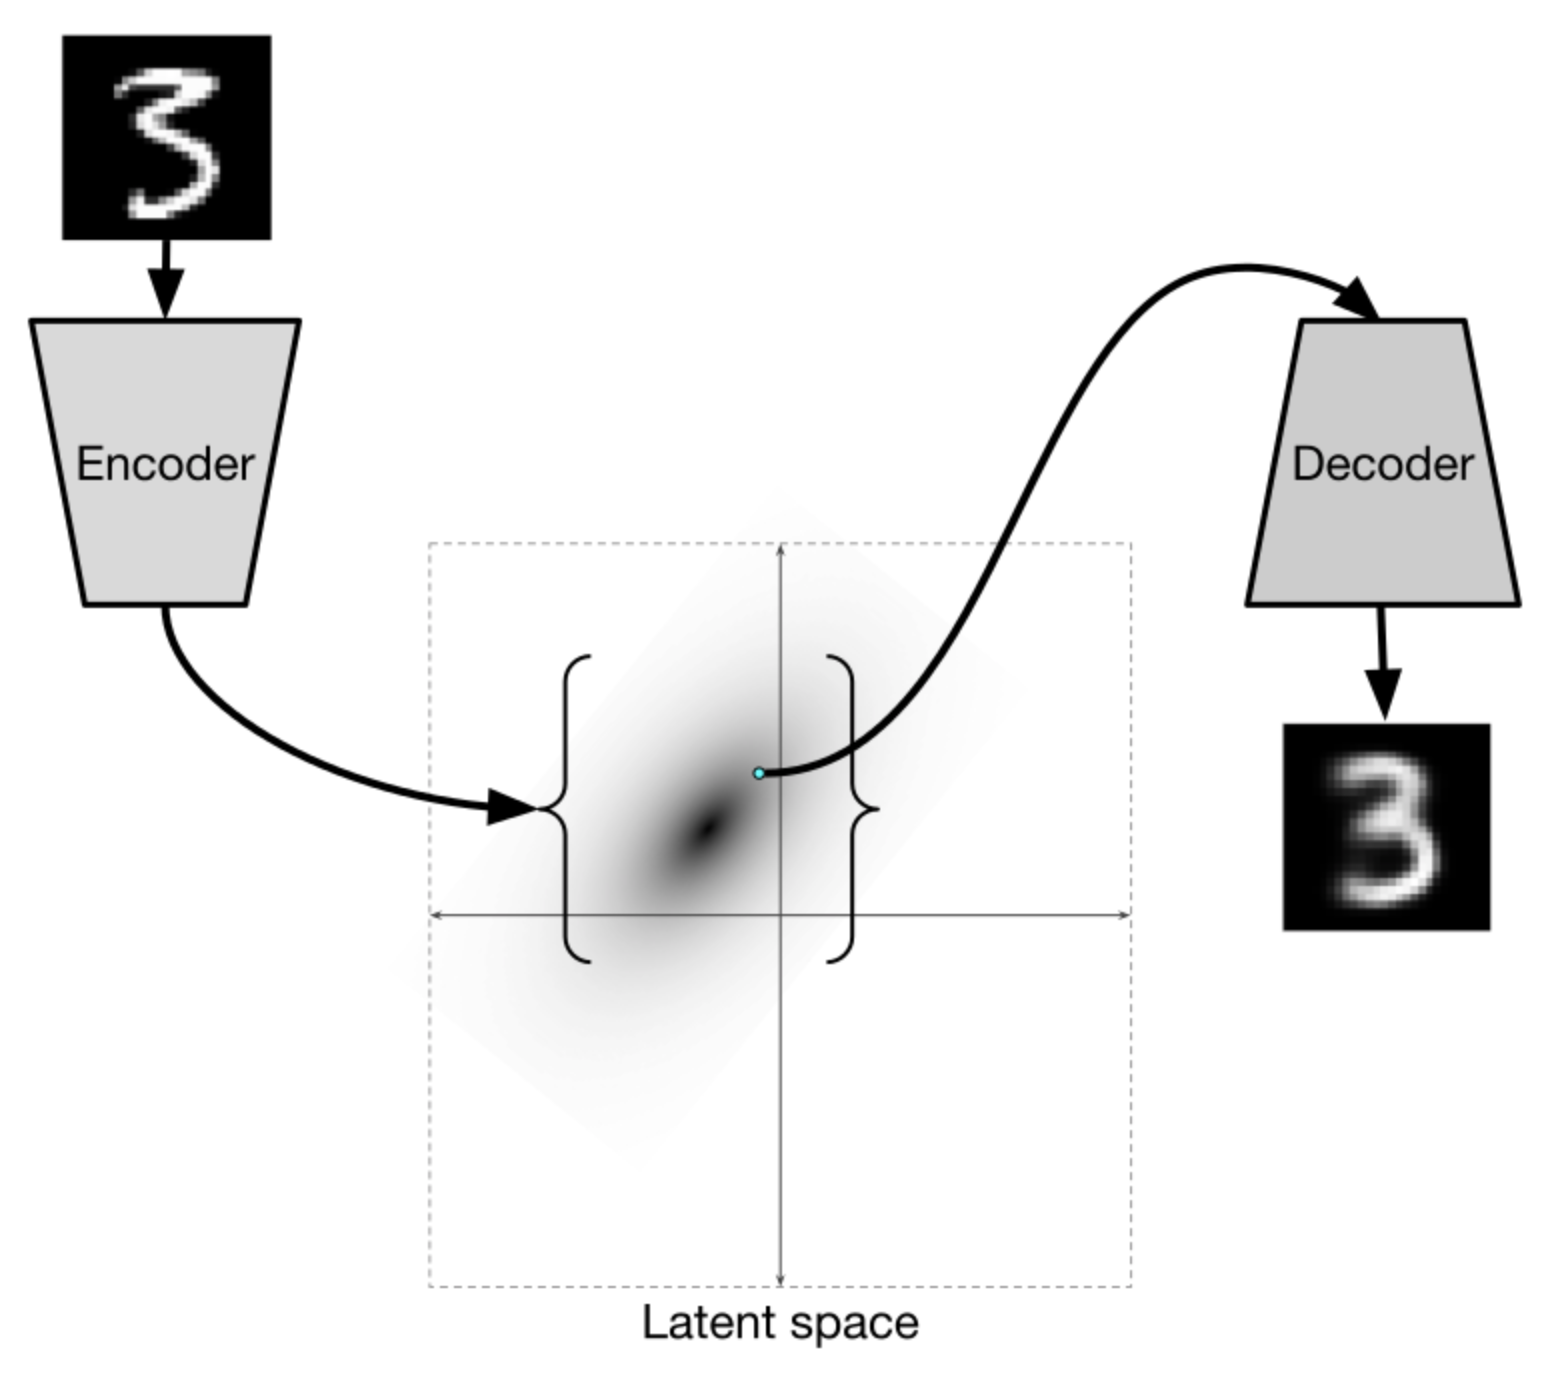
\includegraphics[width=\linewidth]{figs/VAE}
		\end{figure}
	\end{minipage}%
	\begin{minipage}[t]{0.4\columnwidth}
		\begin{figure}[h]
			\centering
			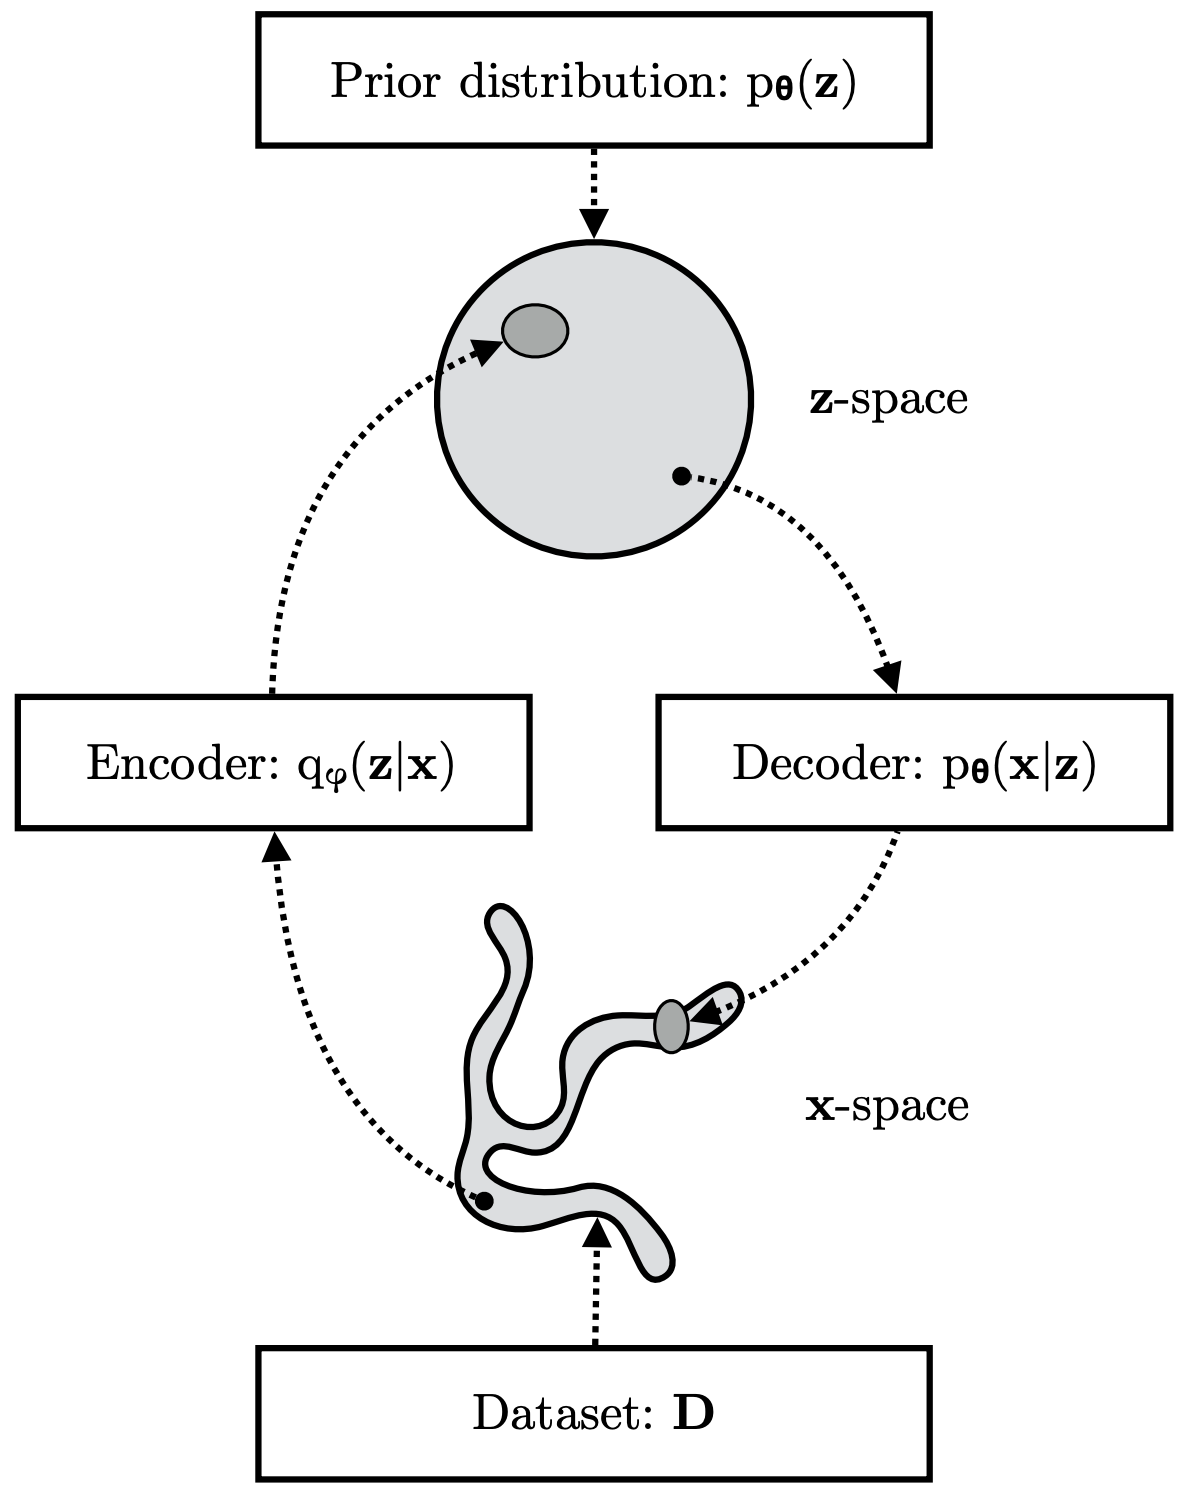
\includegraphics[width=\linewidth]{figs/vae_scheme}
		\end{figure}
	\end{minipage}
	\eqpause
	VAEs are widely used as a preliminary stage of projecting data onto low-dimensional space.
\end{frame}
%=======
\begin{frame}{Variational Autoencoder}
	\myfootnotewithlink{https://arxiv.org/abs/2403.18103}{Chan S., Tutorial on Diffusion Models for Imaging and Vision, 2024}
	\begin{itemize}
		\item The encoder $q_{\bphi}(\bz| \bx) = \NN_{e, \bphi}(\bx)$ outputs $\bmu_{\bphi}(\bx)$ and $\bsigma_{\bphi}(\bx)$.
		\item The decoder $\pt(\bx | \bz) = \NN_{d, \btheta}(\bz)$ outputs parameters of the observed data distribution.
	\end{itemize}
	\begin{figure}[h]
		\centering
		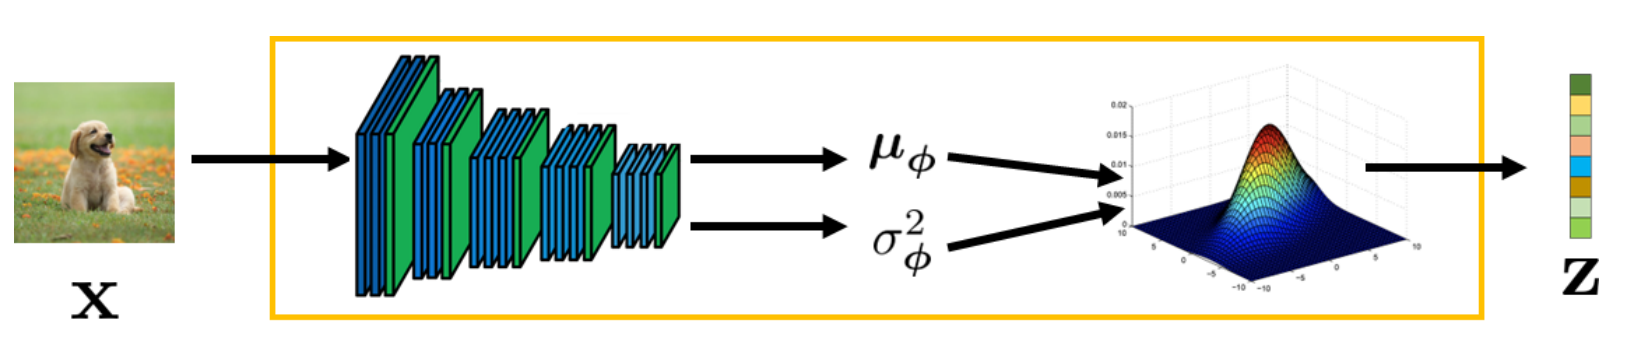
\includegraphics[width=0.7\linewidth]{figs/vae-encoder}
	\end{figure}
	\begin{figure}[h]
		\centering
		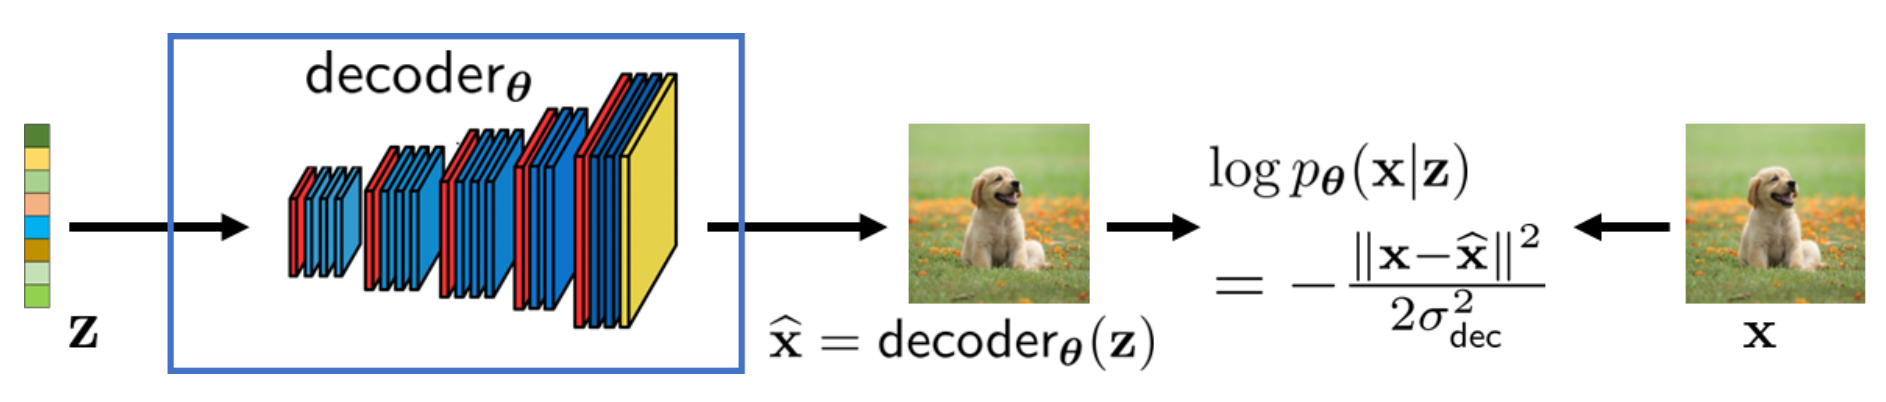
\includegraphics[width=0.9\linewidth]{figs/vae-decoder}
	\end{figure}
\end{frame}
%=======
\begin{frame}{VAE vs Normalizing Flows}
	\myfootnotewithlink{https://arxiv.org/abs/2007.02731}{Nielsen D., et al., SurVAE Flows: Surjections to Bridge the Gap Between VAEs and Flows, 2020}
	\begin{table}[]
		\begin{tabular}{l|c|c}
			& \textbf{VAE} & \textbf{NF} \\ \hline
			\textbf{Objective} & ELBO $\cL$ & Forward KL/MLE \\ \hline
			\textbf{Encoder} & 
			\shortstack{stochastic \\ $\bz \sim q_{\bphi}(\bz| \bx)$} &  
			\shortstack{\\ deterministic \\ $\bz = \bff_{\btheta}(\bx)$ \\ 
			$q_{\btheta}(\bz| \bx) = \delta(\bz - \bff_{\btheta}(\bx))$}  \\ \hline
			\textbf{Decoder} & 
			\shortstack{stochastic \\ $\bx \sim \pt(\bx| \bz)$} & 
			\shortstack{\\ deterministic \\ $\bx = \bff^{-1}_{\btheta}(\bz)$ \\ 
			$ \pt(\bx | \bz) = \delta(\bx - \bff^{-1}_{\btheta}(\bz))$} \\ \hline
			\textbf{Parameters}  & $\bphi, \btheta$ & $\btheta \equiv \bphi$\\ 
		\end{tabular}
	\end{table}
	\vspace{-0.3cm}
	\eqpause
	\begin{block}{Theorem}
		MLE for a normalizing flow is equivalent to maximizing the ELBO for a VAE where:
		\[
			\pt(\bx | \bz) = \delta (\bx - \bff^{-1}_{\btheta}(\bz)); \quad 
			q_{\btheta}(\bz| \bx) = \delta (\bz - \bff_{\btheta}(\bx)).
		\]
	\end{block}
\end{frame}
%=======
\begin{frame}{Summary}
	\begin{itemize}
		\item LVMs maximize the variational evidence lower bound (ELBO) to obtain maximum likelihood estimates for the parameters.
		\vfill
		\item Parametric posterior distribution $q_{\bphi}(\bz| \bx)$ makes the method scalable.
		\vfill
		\item The reparametrization trick provides unbiased gradients with respect to the variational posterior $q_{\bphi}(\bz| \bx)$.
		\vfill
		\item The VAE model is a latent variable model parameterized by two neural networks: a stochastic encoder $q_{\bphi}(\bz| \bx)$ and a stochastic decoder $\pt(\bx | \bz)$.
		\vfill
		\item Nowadays, the main role of VAEs is to project data into low-dimensional latent space.
	\end{itemize}
\end{frame}
\end{document}